\documentclass[jmp, amsmath, amssymb, reprint]{article}

\usepackage[utf8]{inputenc}
\usepackage[english]{babel}
\usepackage{amsmath,graphicx,varioref,verbatim,amsfonts,geometry,grffile}
\usepackage[usenames,dvipsnames,svgnames,table]{xcolor}
\usepackage[colorlinks]{hyperref}
\usepackage{flafter}
\usepackage{float}
\usepackage{placeins}
\usepackage{fancyvrb}
\usepackage{comment}
\usepackage{blindtext}
\usepackage{enumitem}
\usepackage{subcaption}
% Document formatting
\setlength{\parindent}{0mm}
\setlength{\parskip}{1.5mm}
%Color scheme for listings
\usepackage{textcomp}
\definecolor{listinggray}{gray}{0.9}
\definecolor{lbcolor}{rgb}{0.9,0.9,0.9}
%Listings configuration
\usepackage{listings}
%Hvis du bruker noe annet enn python, endre det her for å få riktig highlighting.
\lstset{
	backgroundcolor=\color{lbcolor},
	tabsize=4,
	rulecolor=,
	language=python,
        basicstyle=\scriptsize,
        upquote=true,
        aboveskip={1.5\baselineskip},
        columns=fixed,
	numbers=left,
        showstringspaces=false,
        extendedchars=true,
        breaklines=true,
        prebreak = \raisebox{0ex}[0ex][0ex]{\ensuremath{\hookleftarrow}},
        frame=single,
        showtabs=false,
        showspaces=false,
        showstringspaces=false,
        identifierstyle=\ttfamily,
        keywordstyle=\color[rgb]{0,0,1},
        commentstyle=\color[rgb]{0.133,0.545,0.133},
        stringstyle=\color[rgb]{0.627,0.126,0.941}
        }
        
\newcounter{subproject}
\renewcommand{\thesubproject}{\alph{subproject}}
\newenvironment{subproj}{
\begin{description}
\item[\refstepcounter{subproject}(\thesubproject)]
}{\end{description}}

\lstset{inputpath="C:/Users/Jon Andre/Python/FYS2150"}
\graphicspath{{C:/Users/Jon Andre/Python/FYS2150/Magnetisme/}}
\numberwithin{equation}{section}
\usepackage{dcolumn}% Align table columns on decimal point
\usepackage{bm}% bold math
\usepackage{multicol}
\usepackage{physics}

\newcommand{\e}{\mathrm{e}}
\newcommand{\lp}{\left(}
\newcommand{\rp}{\right)}


\begin{document}

\title{Medical and Biological Physics}

\author{Jon A Ottesen}
%{Institute of physics, University in Oslo}%Lines break automatically or can be 
\title{Compendium FYS3700}% Force line breaks with \\
\date{\today}
\maketitle

\newpage
\tableofcontents
\newpage

\begin{multicols}{2}

\section{Atomic and Molecular physics}

\subsection*{Introduction}

Add introduction

\subsection{Quantum Mechanics}

At macroscopic scale QM becomes absolute but when the scale becomes microscopic QM is necessary to completely describe a system of atoms or molecules. Some solutions for the system is acquired by solving the Hamiltonian operator
\begin{equation}
 \hat{H} = \frac{\hat{p}^2}{2m} + V(\vec{r},t)
\end{equation}
one way or another, this is also known as the time independent Schrödinger equation. Sadly the only exactly solvable atom or molecule is the Hydrogen atom. For all other atoms or molecules consisting of more than a two-atomic system the electron repulsion makes the system \textbf{NOT} exactly solvable and approximations are necessary.

\subsubsection{Hydrogen}\label{sec:hydrogen}

As mentioned earlier the only exactly solvable atomic system is the Hydrogen atom. The solution to the hydrogen atom is given by the wave function\footnote{In QM a wave function is the complete mathematical description of a given system.}
\begin{equation}\label{eq:01}
\Psi\lp n,l,m_l, m_s\rp.
\end{equation}
This means that the complete description of the hydrogen atom depends on four distinct variables all describing different attributes of the atom. Each different combination of these numbers corresponds to a specific allowed state that the Hydrogen atom can take.

From Bohr's description of the hydrogen atom you may recognize the quantum number n. This quantum number indicates which quantized energy eigenvalue corresponds to the given state in the system. This quantized energy is given by
\begin{equation}
E_n = \frac{E_1}{n^2}\quad n=1,2,3,...
\end{equation}
where \(E_1\) is the lowest quantized energy, an important note is that n is only integers which in Bohr's atom model corresponds to a specific shell. Each of these shells are given a name starting at K(\(n=1\)), L(\(n=2\)) etc. Each shell can also hold up to \(2n^2\) electrons, the reason for this will be revealed in the orbitals section.

The second quantum number is l which describes the angular momentum of the system. Again as with the energy states this quantum number also has distinct eigenvalues
\begin{equation}
L = \hbar\sqrt{l\lp l+1\rp} \quad l=0, 1, 2,..., n-1.
\end{equation}
The third quantum number is the magnetic quantum number and gives the value of the angular momentum in the z-direction
\begin{equation}
L_z = \hbar m \quad m=-l, -l+1, ..., 0, ...,l-1, l.
\end{equation}
The last quantum number is $m_s$ and is the spin quantum number of the electron and takes the following values
\begin{equation}
m_s=\pm\frac{1}{2}.
\end{equation}

This might not seem like much but we have now found out that the complete description of the Hydrogen atom\footnote{I know i haven't given you the actual wave function but for out purpose it's unnecessary} only depends on four variables. We have also found both the permitted energy eigenvalues and angular momentum eigenvalues.

So far I haven't really said how the electron configuration is in the Hydrogen atom (or anything really), but I have said that a state of the Hydrogen atom is given by equation \ref{eq:01}. So what is really a state, it's just a possible placement\footnote{Placement is not really the correct word, after all it's really just a probability density.} for an electron in the Hydrogen atom. 

If you have looked closely at the permitted values for the quantum numbers you may have noticed that there are multiple states for each energy level. When multiple different states gives the same eigenvalue we have degeneracy. This degeneracy corresponds to different states an electron can have with said energy level or shell if you will. Meaning that there are multiple possible placements for an electron in each energy level or shell. This is important when describing the amount of electrons an atom can take in it's outer shell.

\subsubsection{Orbitals}

A orbital is a designation of the combination of quantum numbers that gives the state of the electron. These orbitals are categorized after which n and l value the state is in, the shape is also determined by the angular momentum quantum number l. Some orbital names are shown in table \ref{tabel:1}. By counting the different states in each orbital lets say 2p you find that there are a total of $m_s=-1, 0, 1$ magnetic states each with two different spins and therefore a total of 6 states in the 2p orbital. Each orbital does not only have different amounts possible electron states but the probability density also vary greatly as seen in figure \ref{fig:orbitals}.

\begin{table}[H]
  \begin{center}
    \begin{tabular}{| l | l | l | l | l |}
   	\hline
	 & \(l=0\) & \(l=1\) & \(l=2\) & \(l=3\)\\ \hline
	\(n=1\) & 1s &  &  & \\
	\(n=2\) & 2s & 2p &  & \\
	\(n=3\) & 3s & 3p & 3d & \\
	\(n=4\) & 4s & 4p & 4d & 4f\\ \hline
	\end{tabular}
    \caption{The different orbitals for each energy level and angular momentum.}
    \label{tabel:1}
  \end{center}
\end{table}
\FloatBarrier

\begin{figure}[H]
	\centering
  	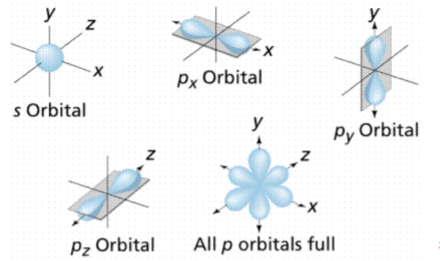
\includegraphics[width=0.55\textwidth]{orbitals.png}
	\caption{The different shape of the s and p orbitals, the direction is determined by the magnetic quantum number \(m_l\).}
	\label{fig:orbitals}
\end{figure}

In the 2p orbital you already know that there are a total of 6 possible states or different electron combinations but does this mean that the orbital 2p can maximum accept 6 electrons? Can electrons share the same quantum numbers? The answer is \textbf{NO}. This comes from The Pauli principle: \textit{Two electrons cannot share all four quantum numbers}. This is important, let's for a moment imagine two hydrogen atom binding together. The Pauli principle than states that the electrons in this molecule cannot share the same quantum number but they can be degenerate (different spin) within the same \(l\) and \(m_l\) values. 

So far i haven't stated where electron prefer to be located. I won't elaborate much on this but they follow the principle of minimum energy, meaning that the electrons seek their lowest possible energy. In the \(H_2\) case this is the 1s orbital, this also means that the electrons fill up the orbitals with the minimum energy first\footnote{I won't elaborate much on this, but for us this means that electrons will fill up the orbitals 1s, 2s, 2p, 3s, 3p. The rest is not ordered as you would think from table \ref{tabel:1}, see internet.} in a given molecule. If you f.eks were asked to give the orbital configuration of Aluminum it would be: \(1s^2, 2s^2, 2p^6, 3s^2\) and \(3p^1\).

So far you know that that the orbitals are filled from the lowest energy and upwards but not how each orbital is filled. Another way of phrasing this is; which combination of the magnetic $m_l$ and spin $m_s$ quantum numbers would be used firstly to fill a orbital. To solve this we have Hund's rule: \textit{Electrons fill their states (orbitals) with as many parallel spins as possible}. In simpler terms this means that the 2p orbital would first fill all the $m_l$ values with spin \(m_s=\frac{1}{2}\) before filling up any \(m_l\) with spin with \(m_s=-\frac{1}{2}\)\footnote{When I say that \(m_s=\frac{1}{2}\) is filled up firstly this is just a convention that spin up is filled firstly.}. An illustration of this is shown in figure \ref{fig:orbitals}.

\begin{figure}[H]
	\centering
  	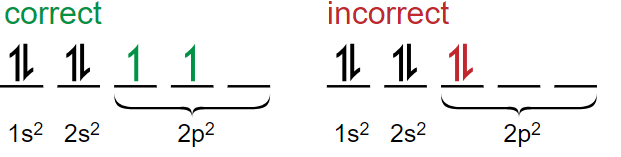
\includegraphics[width=0.50\textwidth]{hunds_rule.png}
	\caption{An illustration of Hund's rule.}%https://ch301.cm.utexas.edu/svg/hunds-rule.svg
	\label{fig:orbitals}
\end{figure}

\subsection{Atomic and molecular bonds}

\subsubsection{Chemical bonds}

For most of you this subsection might seem redundant since it will only cover the very basics but bonds are such a fundamental part of all macroscopic matter so it's absolutely a necessity.

Chemical bonds are often categorized by the strength of the bond. The bonds where there are needed large amount of energy the break the bond is considered strong while the weak bonds require less. The strong bonds are bonds that creates molecular structures through covalent bonds or crystal structure through ionic bonds. Weaker bonds are to weak to connect atoms together and instead work between molecules and create a more macroscopic structures. Weaker bonds are divided into polar, hydrogen and van der Waals bonds. To get a feel for the different distances and strength values see table \ref{tabel:2}.

\begin{table}[H]
  \begin{center}
    \begin{tabular}{| l | l | l |}
   	\hline
	Bonding type & length [nm] & Strength [kcal/mol] \\ \hline
	Covalent & 0.15 & 90\\
	Ionic & 0.25 & 3\\
	Hydrogen & 0.30 & 1\\
	van der Waals & 0.35 & 0.1\\ \hline
	\end{tabular}
    \caption{The strength and distance for the different types of bonds in.}
    \label{tabel:2}
  \end{center}
\end{table}
\FloatBarrier

Covalent bonds are bonds between atoms or between molecules and atoms forming molecules. When two atoms are bonded together with at covalent bond they share an electron pair and the repulsive and attractive forces are stable. This happens to the atoms when their electronegativity\footnote{'Electronegativity is a measure of the tendency of an atom to attract a bonding pair of electrons', try searching for a table you might find some pattern with where the electronegativity is largest and smallest.} is identical or relatively close. The physical reason for creating these bonds are to minimize the total energy of the system. Meaning that the total energy for a bonded molecule is less than if the atoms were roaming free without a full outer shell. Covalent bonds are again divided into two types of bonds sigma and pi bonds which we will discuss again later in the hybridization subsection.

Ionic bonds unlike covalent bonds doesn't share their respective electrons between atoms but instead transfer\footnote{Completely transfer of electrons in ionic bonds doesn't exist but the electronegativity will force the electron closer to one atom.} electrons to each other. This means that this bonding type require both a transfer atom and a receiver atom for the electron(s). This happens thanks to a large difference in electronegativity larger than \(1.7\) between the atoms, and we therefore have Coulomb interactions which stabilizes the structure. Much like covalent bonds this bond does also minimize the total energy of the system\footnote{When saying system I usually refer to a general system of a couple of atoms.}. Ionic bonds unlike covalent bonds can create macroscopic structures in the form of crystals like table salt NaCl. These structures have a high smelting point thanks to the high bond strength.

Polar bonds are a type of bonds which happens without any transfer or sharing of electrons. It's actually a weaker version of ionic bonds where the electrons isn't transferred. More specifically polar bonds occur when the electronegativity is smaller than \(1.7\). Polar bonds therefore often occur between molecules where the charge of the electrons are unevenly distributed between the atoms thanks the the difference in electronegativity in the atom. The polar part of the molecule is designated by the letter \(\delta^+\) while the negative is by \(\delta^-\). Most macroscopic structures are made up of molecules bonded together by the polar bonds between the molecules. A example of a macroscopic structure is water \(H_2O\), without the polar bonds there would be no water. A good analogy for polar bonds is to think of the molecules as microscopic magnets that attract each other and then forms a macroscopic structure thanks to the attractive forces. 

Hydrogen bonds are a \textbf{VERY} important sub-type of polar bonds often categorized as it's own type of chemical bond. The very reason being that hydrogen bonds are present in many of the most important structures to humans for example water. Hydrogen bonds occur as with polar bonds when there is a substantial difference between the electronegativity of a hydrogen in a molecule and another atom. This creates a \(\delta^+\) and a \(\delta^-\) making it possible to have electromagnetic forces keeping other types of polar molecules together. Example with a water (\(H_2O\)): The electronegativity of oxygen is 3.5 while hydrogen has 2.1. The oxygen will therefore have a greater pull on the electrons and it will be negatively charged compared to the hydrogen atoms. This results in two positively charges hydrogen atoms and one negatively charged oxygen atom. This results in a hydrogen bond between hydrogen and oxygen from different molecules thanks to Coulomb interactions. The hydrogen bond in water is depicted in figure \ref{fig:hydrogen_bond}.

\begin{figure}[H]
	\centering
  	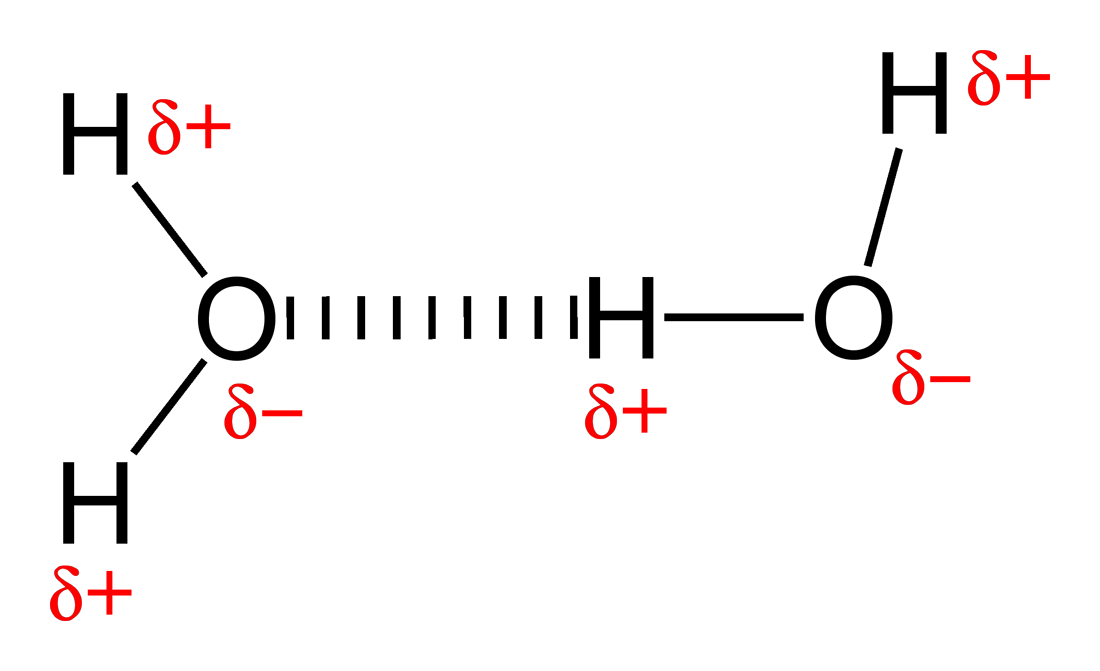
\includegraphics[width=0.50\textwidth]{hydrogen_bond.png}
	\caption{An illustration of Hund's rule.}%https://commons.wikimedia.org/wiki/File:Hydrogen-bonding-in-water-2D.png
	\label{fig:hydrogen_bond}
\end{figure}

Van der Waals bonds are a special kind of snowflake when it comes to binding. They are clearly the weakest type of bonds but are still important when maintaining the structure when the molecules are non-polar. An example of non polar molecules are multiple gasses in the air \(O_2\), \(CO_2\) etc. Van der Waals bonds are weak interactions between molecules without any notable permanent dipolar moment\footnote{Dipolar moment is another way of defining the difference between the electronegativity within a molecule.}. So what are these weak interactions? From earlier QM courses you should know that the positions of electrons are given as probability densities located around the the atomic nucleus. This also means that the electrons aren't at a fixed location. A result of this is that the electrons can be heavily located at a certain section within the molecule. A high density of electrons in a specific area creates a net negative charge at a fixed position and as a result a net positive charge is created another place in the molecule. We therefore have a temporary dipole moment, which is used to form bonds with other temporary dipole moments. A general way of defining van der Waals are that they are created by temporary fluctuations in the charge distribution.

\subsubsection{Hybridization}

''Hybridization is Man’s way of mathematically being able to describe Mother Nature’s inherent need for a minimalization of the total energy for a given system.''

Hybridization is the concept of mixing atomic orbitals. A general definition of hybridization of orbitals is that they are a linear combination of the x states involved in the molecular structure, and the result is x new linearly independent, orthogonal states. The QM way of describing this would be
\begin{equation}\label{eq:02}
\Psi = \sum_{i=0}^N c_i\psi_i
\end{equation}
where \(\Psi\) is the new wave function for the molecule built up of N weighted \(c_i\) \(\psi\) states from other states. It's important to state that this is just an approximation since it's impossible to completely solve a more than two atomic system. Still this approximation closely resemble that of mother nature. So it's a model, but a good one!

I will now for the 'simple' \(H_2\) molecule use QM and hybridization to showcase the basics of hybridization. I firstly need to consider two hydrogen atoms A and B both in the s orbital that bonds together to the \(H_2\) molecule. Form hybridization this is then a linear combination of the states of A and B, from equation \ref{eq:02} this is normalized
\begin{align}
\Psi_{AB+} = d_{AB}\lp c_A\psi_A + c_B\psi_B\rp\label{eq:03}\\
\Psi_{AB-} = d_{AB}\lp c_A\psi_A - c_B\psi_B\rp.\label{eq:04}
\end{align}
An important note is that in equation \ref{eq:02} I don't exclude negativity as seen in the linear combination above. An illustration is shown in figure \ref{fig:wave_sum} where you can see how the electron density behaves depending on the sign in the wave function. 

\begin{figure}[H]
	\centering
	\begin{subfigure}{0.49\textwidth}
  	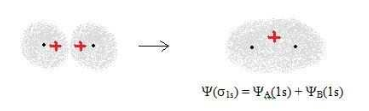
\includegraphics[width=1\textwidth]{h2_pos.png}
	\caption{Equation \ref{eq:03}.}
	\end{subfigure}
	\begin{subfigure}{0.49\textwidth}
  	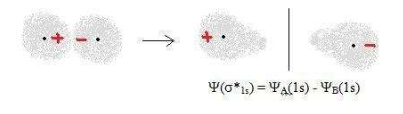
\includegraphics[width=1\textwidth]{h2_neg.png}
	\caption{Equation \ref{eq:04}.}
	\end{subfigure}
	\caption{An illustration on how the electron density behaves at different signs.}
	\label{fig:wave_sum}
\end{figure}

There is a couple points of importance from figure \ref{fig:wave_sum} and thereby with equation \ref{eq:03} and \ref{eq:04}. Equation \ref{eq:03} gives high electron density in the middle of the nuclei and the atoms share bonding orbitals. In equation \ref{eq:04} the electron density is lower and there are no shared orbitals. This leads to two different types of bonds between the atoms, the regular bond which belongs to equation \ref{eq:03} and one anti-bond which belongs to equation \ref{eq:04}. Regular bonds are more stable and have a low internal energy while anti-bonds are unstable and their energy is higher than when separated. The energy differences can be seen in figure \ref{fig:bond_energy}. It's important to know that anti-bonding and bonding isn't classification on the type of covalent bonds, but rather the composition of the wave function. A general way of though is that negative signs corresponds to repulsion of the electrons densities in regards to one another. A mathematical proof for the difference in energy between anti and regular bonds can be found in...

\begin{figure}[H]
	\centering
  	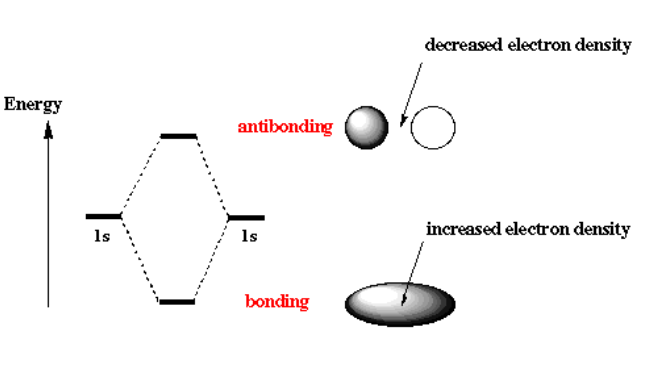
\includegraphics[width=0.50\textwidth]{anti_bond_energy.png}
	\caption{A illustration of the energy difference between anti-bonds and regular bonds.}
	\label{fig:bond_energy}
\end{figure}

Covalent bonds are separated into two different types: \(\sigma\) and \(\pi\) bonds. Both of these bonding types occure both as anti and regular bonds, meaning you can have an anti \(\sigma\) bond. These bonds are separated by how the orbitals are situated. Sigma bonds are bonds created by overlapping of orbitals. The definition is that: \(\sigma\)-bonds are bonds where the orbitals are symmetric with respect to the molecular axis\footnote{The axis between the nuclei the bond is formed.}. This means that sigma bonds can be created by both a mixture of s, p, d etc orbitals as long as the linear combination is symmetric, this is shown in figure \ref{fig:sigma_bonds}. A \(\pi\)-bond is a bond defined as: A \(\pi\)-bond is asymmetric with respect to the nodal plane\footnote{The nodal plane is a plane where the electron density is zero, in this case on the molecular axis.}. \(\pi\) bonds are weaker than \(\sigma\)-bonds since their overlapping of orbitals are less prominent. A example of \(\pi\)-bonds are shown in figure \ref{fig:pi_bonds}. In the figure I have also shown anti \(\pi\)-bonds, these are asymmetric around both axes shown in the figure, the difference in sign on the figure is a result of the sign difference in the wave function.


\begin{figure}[H]
	\centering
  	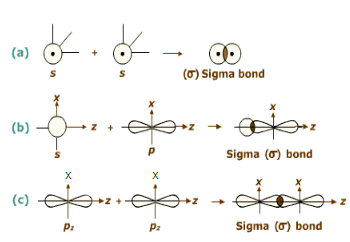
\includegraphics[width=0.50\textwidth]{sigma_bonds.png}
	\caption{\(\sigma\)-bonds between diffrent orbitals.}
	\label{fig:sigma_bonds}
\end{figure}

\begin{figure}[H]
	\centering
  	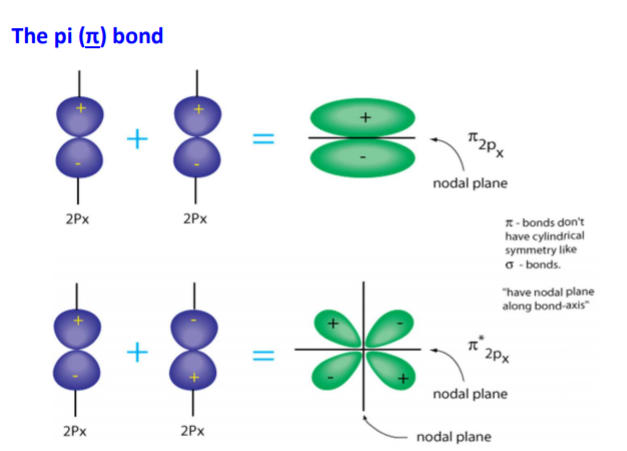
\includegraphics[width=0.50\textwidth]{pi_bonds.png}
	\caption{Both \(\pi\)-bonds and anti \(\pi\)-bonds.}
	\label{fig:pi_bonds}
\end{figure}

\subsubsection{sp - sp\(^2\) - sp\(^3\) hybridization}

We will here look at three different hybridization types that are essential in organic material. When finding the hybrid orbital made up of different orbitals the new hybrid orbital will have new energy that is between that of the originals as illustrated in figure \ref{fig:hybrid_energy}. When a hybrid orbital is created on a atom that is bonding with other atoms the hybrid orbital is a linear combination of different states on the bonding atom.

\begin{figure}[H]
	\centering
  	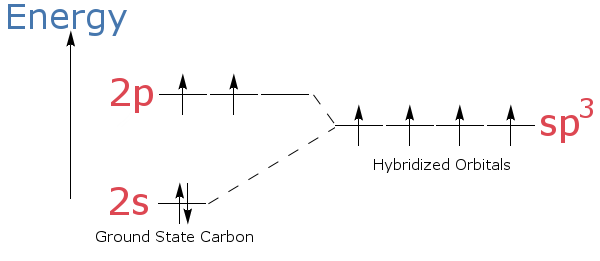
\includegraphics[width=0.50\textwidth]{hybrid_orbital_energy.png}%https://www.chemicool.com/img1/graphics/sp3energylevels1.png
	\caption{Illustration on how the energy is for a hybrid orbital compared to that of the originals.}
	\label{fig:hybrid_energy}
\end{figure}

Sp hybridization is a type of hybridization that occurs when combing the 2s orbital with one 2p orbital. This results in two new sp hybrid orbitals while the atom keeps two p orbitals. The wave functions for sp orbitals are
\begin{align}
\Psi_1 = \frac{1}{\sqrt{2}}\lp \psi_{2S}+\psi_{2px}\rp\\
\Psi_2 = \frac{1}{\sqrt{2}}\lp \psi_{2S}-\psi_{2px}\rp.
\end{align} 
The sp orbitals are located at the same axis while the two p-orbitals are standing perpendicular on this axis and on each other. An example on sp hybridization is shown in figure \ref{fig:sp_orbital}. As seen on the figure this produces two \(\pi\)-bonds between the p-orbitals on the carbon atoms. A general rule is that with triple bindings between carbon is that it's sp hybridized and therefore two of these bindings are \(\pi\)-bonds.

\begin{figure}[H]
	\centering
  	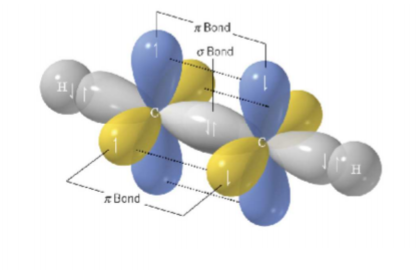
\includegraphics[width=0.50\textwidth]{sp_orbital.png}
	\caption{Sp hybridization on ethyne \(C_2H_2\).}
	\label{fig:sp_orbital}
\end{figure}

Sp\(^2\) hybridization is a type of hybridization that occurs when combing one 2s orbital with two 2p orbitals. This results in three new sp\(^2\) hybrid orbitals while one p orbital still remain. The wave functions for sp\(^2\) orbitals are
\begin{align}
\Psi_1 = \frac{1}{\sqrt{3}}\lp \psi_{2S}+\sqrt{2}\psi_{2px}\rp\\
\Psi_2 = \frac{1}{\sqrt{3}}\lp \psi_{2S} -\frac{1}{\sqrt{2}}\psi_{2px} + \frac{\sqrt{3}}{\sqrt{2}}\psi_{2py}\rp\\
\Psi_3 = \frac{1}{\sqrt{3}}\lp \psi_{2S} -\frac{1}{\sqrt{2}}\psi_{2px} + \frac{\sqrt{3}}{\sqrt{2}}\psi_{2py}\rp.
\end{align}
The sp\(^2\) orbitals are arranged in a triangular shape on the same plane with angles \(120^\circ\) between. The last p orbital is perpendicular to said plane. An example of a sp\(^2\) hybridized molecule is \(C_2H_4\) which is shown in figure \ref{fig:sp2_orbital}. The triangular shape of the sp\(^2\) orbitals are very important for the general shape of molecules as seen in the figure. A general rule is that for sp\(^2\) hybridization it's one \(\pi\) and one \(\sigma\) bond between the carbon atoms.

\begin{figure}[H]
	\centering
  	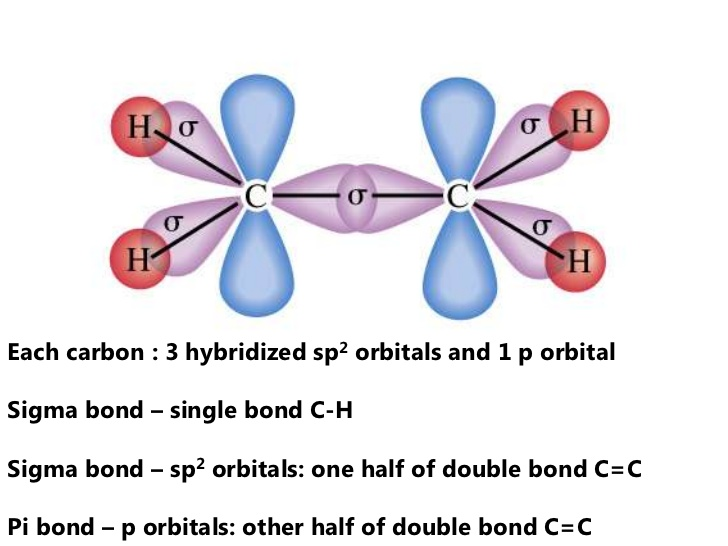
\includegraphics[width=0.50\textwidth]{sp2_orbital.png}%https://www.slideshare.net/pedagogics/2012-orbital-hybrization-sigma-and-pi-bonds
	\caption{Sp\(^2\) hybridization on ethene \(C_2H_4\).}
	\label{fig:sp2_orbital}
\end{figure}

Sp\(^3\) hybridization is a type of hybridization that occurs when combing one 2s orbital with three 2p orbitals. This results in four new sp\(^3\) hybrid orbitals with no remaining p orbitals. The wave functions for sp orbitals are
\begin{align}
\Psi_1 = \frac{1}{2}\lp \psi_{2s} + \psi_{2px} + \psi_{2py} + \psi_{2pz}\rp\\
\Psi_2 = \frac{1}{2}\lp \psi_{2s} + \psi_{2px} - \psi_{2py} - \psi_{2pz}\rp\\
\Psi_3 = \frac{1}{2}\lp \psi_{2s} - \psi_{2px} + \psi_{2py} - \psi_{2pz}\rp\\
\Psi_4 = \frac{1}{2}\lp \psi_{2s} - \psi_{2px} - \psi_{2py} + \psi_{2pz}\rp.
\end{align}
The sp\(^3\) orbitals are arranged in a tetrahedral shape on the same plane with a angel \(\approx 109^\circ\) between. An example of a sp\(^3\) hybridized molecule is \(C_2H_4\) which is shown in figure \ref{fig:sp3_orbital}. The tetrahedral shape of the sp\(^3\) orbitals are important for the general shape of molecules as seen in the figure. For sp\(^3\) there are only \(\sigma\)-bonds between the atoms.

\begin{figure}[H]
	\centering
  	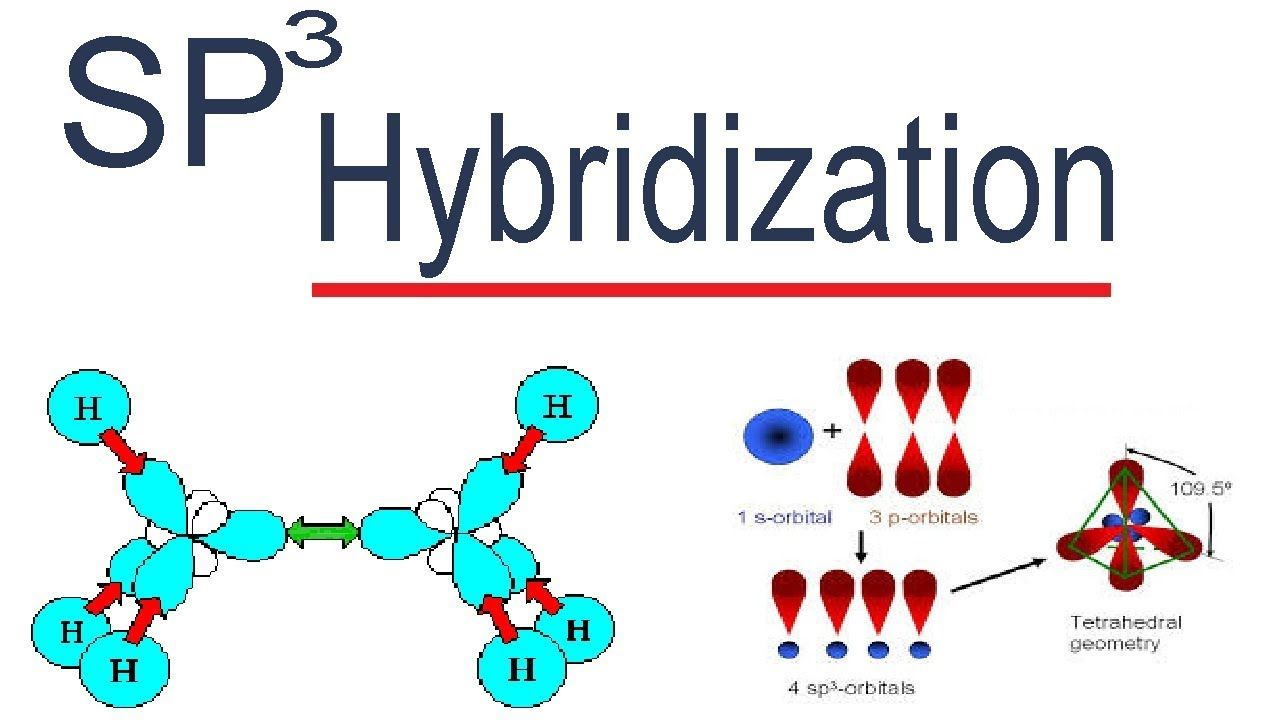
\includegraphics[width=0.50\textwidth]{sp3_orbital.png}%https://i.pinimg.com/originals/bc/9b/e4/bc9be459f7c5bb02c204f35ca16fd2c0.jpg
	\caption{Sp\(^3\) hybridization on ethane \(C_2H_6\).}
	\label{fig:sp2_orbital}
\end{figure}

\clearpage

\section{Radioactivity}

\subsection*{Introduction}

Add introduction

\subsection{Radiation}

Radiation is the emission or transmission of energy in the form of waves or particles. The transmission of energy in waves are through electromagnetic radiation like: gamma, x-ray, ultraviolet, visible light etc. The energy of electromagnetic radiation is given by
\begin{equation}
E=h\nu \qquad \nu = \frac{c}{\lambda}.
\end{equation}
The transmission of energy through particles are typically from: alpha particles, electrons, positions, protons etc.

The energy transmitted through radiation is relatively small compared to energy measured on macroscopic systems. Therefore it's advantageous to change units to electron volt instead of the regular joule where
\begin{equation}
1\text{eV}=1.6\cdot 10^{-19}\text{joule}.
\end{equation}
The advantage of using eV can be seen in the rest energy of some particles in table \ref{tabel:3}. The rest energy seen in the table is given by
\begin{equation}
E_0=m_0c^2
\end{equation}
while the relativistic rest energy for a object in motion is
\begin{equation}
E_0=m_0c^2\qquad m=\dfrac{m}{1-\lp\frac{v}{c}\rp}.
\end{equation}
Lastly the total energy is given by
\begin{equation}
E^2=\lp pc\rp^2 + \lp m_oc^2\rp^2\qquad p=\frac{m}{\sqrt{1-\lp\frac{v}{c}\rp^2}}
\end{equation}

\begin{table}[H]
  \begin{center}
    \begin{tabular}{| l | l | l |}
   	\hline
	Particle & Rest mass [kg] & Rest energy [MeV]\\ \hline
	Electron & \(9.11\cdot10^{-31}\) & \(0.511\)\\
	Proton & \(1.67\cdot10^{-27}\) & \(938\)\\
	Neutron & \(1.67\cdot10^{-27}\) & \(938\)\\
	Alpha particle & \(6.64\cdot10^{-27}\) & \(3727\)\\ \hline
	\end{tabular}
    \caption{The different mass and rest energy of a couple of particles.}
    \label{tabel:3}
  \end{center}
\end{table}

From section \ref{sec:hydrogen} you should already know that the hydrogen atom has quantized energy states. The quantized trait is actually more general, and all atoms have quantized energy states. This is the reason for the shell categorization and the principle behind the Bohr atomic structure with the nucleus at the center surrounded by shells housing the electrons.

The fact that the energy of the electrons are quantized leads to many interesting consequences. The most important for us is the fact that the energy emitted thorough electromagnetic radiation is equal to the gap in energy between two shells. The electromagnetic transition between the shells in hydrogen and tungsten is shown in figure \ref{fig:el_transition}, it's not important to know anything specific for these two. But rather that the transitions are random from the n-th energy level down to the lowest possible energy state but the transition is always to a shell with lower energy. Whenever a electron transitions from a higher shell to a lower the energy difference is emitted through electromagnetic radiation.

\begin{figure}[H]
	\centering
  	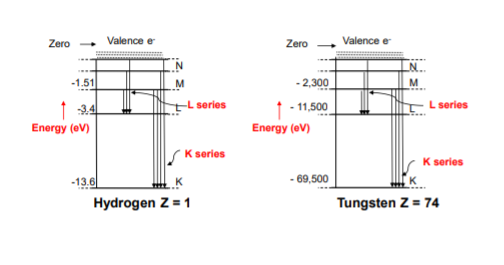
\includegraphics[width=0.50\textwidth]{electromagnetic_transistion.png}
	\caption{The electromagnetic transitions between the shells in hydrogen and tungsten.}
	\label{fig:el_transition}
\end{figure}

\subsection{Ionization}

Ionization is the process by which an atom or a molecule acquires a negative or positive charge by gaining or losing electrons to form ions. In our case when referring to ionization we mostly refer to the process when the atom/molecule gains a positive charge and therefore losses an electron.

Ionization can happen though radiation when the energy of the radiation (particles or EM) is greater or equal to the absolute energy of the electron with the maximum energy. Mathematically this relation is
\begin{equation}
0 \leq E_r + E_n
\end{equation}
where \(E_r\) is the energy of the radiation and \(E_n\) is the energy of the electron. A couple of these energy levels are shown in table \ref{tabel:4}. When ionizing an atom the total energy is conserved. Therefore the total energy before the ionization equals the energy of the ionized electron plus the energy of the ionizing particle or photon after the ionization, mathematically:
\begin{equation}
E_{in} = E_{e-} + E_{p/f}.
\end{equation}


\begin{table}[H]
  \begin{center}
    \begin{tabular}{| l | l |}
   	\hline
	Element & Ionization potential [eV]\\ \hline
	H & 13.6\\
	He & 24.5\\
	C & 11.3\\
	O & 13.6\\
	Mo & 7.1\\
	W & 7.9\\
	H\(_2\)O & 12.6\\ \hline
	\end{tabular}
    \caption{A couple of ionization potentials.}
    \label{tabel:4}
  \end{center}
\end{table}

The minimum energy required for ionization doesn't represent how easy an atom or molecule is ionized. Instead we use the mean excitation energy which measure the mean energy required for ionization of a certain material. Some mean excitation energies is given in table \ref{tabel:5}, notice how they are larger than the potentials given in table \ref{tabel:4}. The mean excitation potentials roughly scales with
\begin{equation}
\left<E_{mean}\right>\sim 10Z
\end{equation}
where Z is the atomic number.

\begin{table}[H]
  \begin{center}
    \begin{tabular}{| l | l |}
   	\hline
	Element & Mean excitation energy [eV]\\ \hline
	H & 19\\
	C & 81\\
	Pb & 823\\
	H\(_2\)O & 75\\ \hline
	\end{tabular}
    \caption{A couple of mean ionization potentials.}
    \label{tabel:5}
  \end{center}
\end{table}

Not all radiation leads to ionization. Rather most radiation leads to a process called excitation. Excitation happens when the electromagnetic radiation equals the energy difference between a bound electron (an electron within a orbital in the atom or molecule) and a higher shell or orbital and hits the electron. When this happens the electron elevates to a higher shell or preferably called state. If you remember the principle of minimum energy you should also know that the electron prefers a state with the minimum energy. Therefore the electron goes through a process called de-excitation. When this happens the electron 'jumps' to a state with lower energy and the difference in energy is released in the form of electromagnetic radiation. The amount of states lowered towards it's minimum energy is random so multiple photons can be released during the de-excitation as stated in the beginning of the radiation section.

Useful quantities:
\begin{enumerate}
\item \(N_A\): Avogadro constant
\item \(A_r\): Atomic weight
\item \(Z\): Atomic number
\item \(\rho\): Density
\item 1 amu: \(1/12\) of the mass of a \(^{12}\)C atom.
\end{enumerate}



\end{multicols}

%\appendix
%\section{Appendix}

%\begin{align}
%\left<E_+\right> = \mel{\Psi_{AB+}}{\hat{H}}{\Psi_{AB+}}\label{eq:03}\\
%\left<E_-\right> = \mel{\Psi_{AB-}}{\hat{H}}{\Psi_{AB-}}\label{eq:04}
%\end{align}

%Following the calculations from equation \ref{eq:03}
%\begin{align}
%\left<E_+\right> = \mel{\Psi_{AB+}}{\hat{H}}{\Psi_{AB+}}\\
%=\lp |c_A|^2\mel{\psi_{A}}{\hat{H}}{\psi_{A}} + |c_B|^2\mel{\psi_{B}}{\hat{H}}{\psi_{B}} + c_A^*c_B\mel{\psi_{A}}{\hat{H}}{\psi_{B}} + c_B^*c_A\mel{\psi_{B}}{\hat{H}}{\psi_{A}}\rp.
%\end{align}
%In this case the Hamiltonian is
%\begin{equation}
%\hat{H} = \hat{H}_0 - V_e + V_p
%\end{equation}
%where \(V_p\) is the potential from the other proton and \(V_e\) is the potential from the other electron.


%\onecolumngrid

%\bibliographystyle{plain}
%\bibliography{referanser} 

\end{document}

